\documentclass{standalone}
\usepackage{tikz}
\usetikzlibrary{patterns, positioning}


\begin{document}
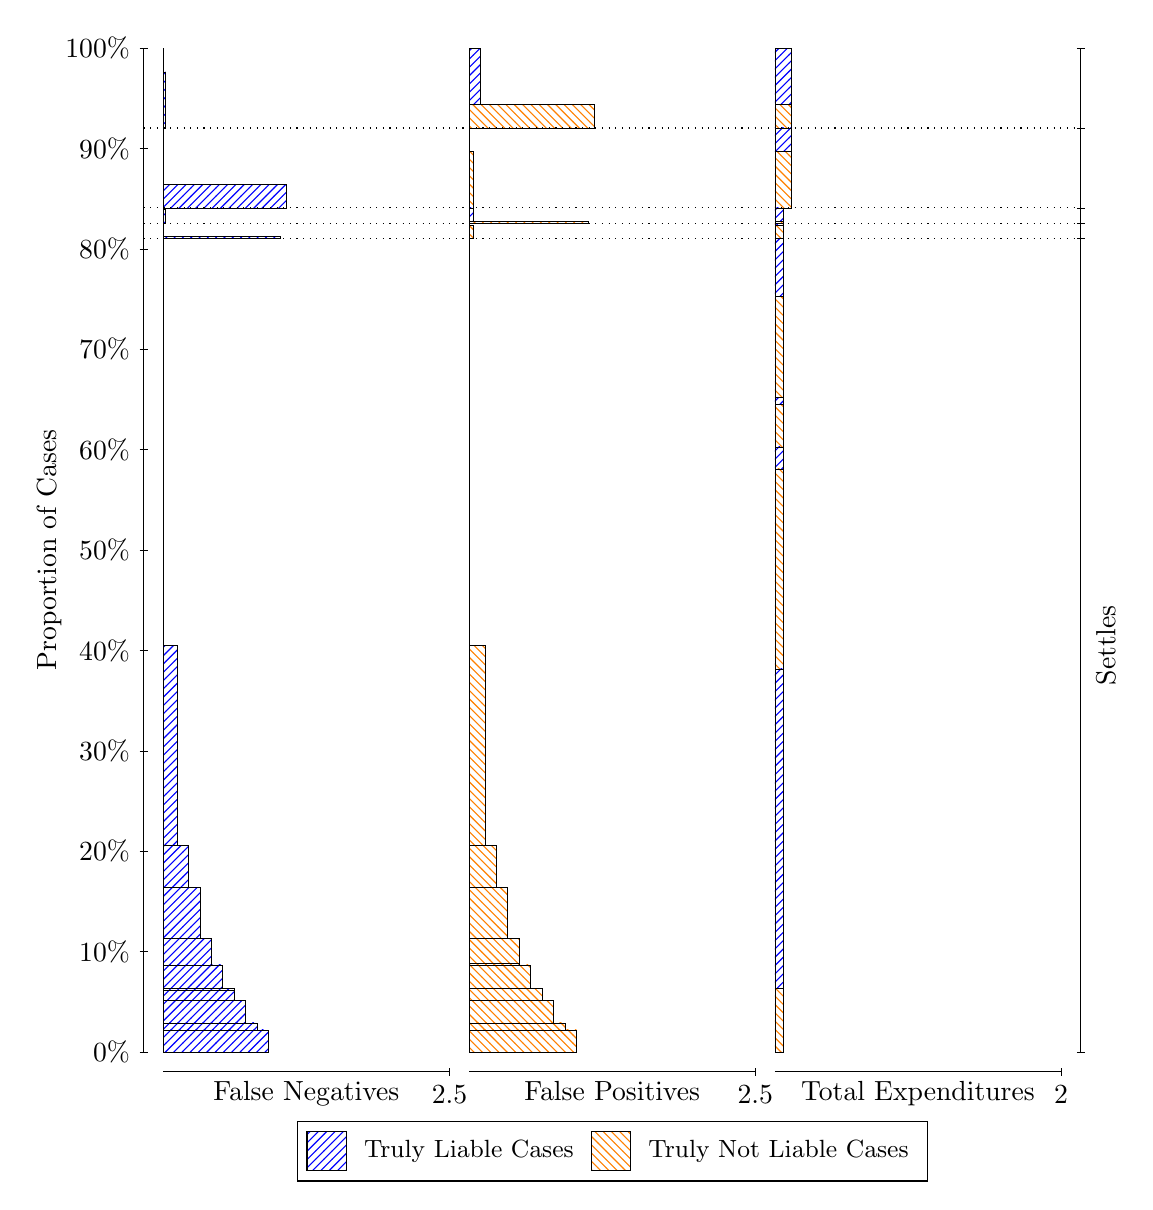
\begin{tikzpicture}
\draw[black, very thin] (1.5,1.75) -- (1.5,14.5);
\node[rotate=90, text=black, anchor=center] at (0.3, 8.125) {Proportion of Cases};
\draw[black, very thin] (1.45,1.75) -- (1.55,1.75);
\node[text=black, anchor=east] at (1.45, 1.75) {0\%};
\draw[black, very thin] (1.45,3.025) -- (1.55,3.025);
\node[text=black, anchor=east] at (1.45, 3.025) {10\%};
\draw[black, very thin] (1.45,4.3) -- (1.55,4.3);
\node[text=black, anchor=east] at (1.45, 4.3) {20\%};
\draw[black, very thin] (1.45,5.575) -- (1.55,5.575);
\node[text=black, anchor=east] at (1.45, 5.575) {30\%};
\draw[black, very thin] (1.45,6.85) -- (1.55,6.85);
\node[text=black, anchor=east] at (1.45, 6.85) {40\%};
\draw[black, very thin] (1.45,8.125) -- (1.55,8.125);
\node[text=black, anchor=east] at (1.45, 8.125) {50\%};
\draw[black, very thin] (1.45,9.4) -- (1.55,9.4);
\node[text=black, anchor=east] at (1.45, 9.4) {60\%};
\draw[black, very thin] (1.45,10.675) -- (1.55,10.675);
\node[text=black, anchor=east] at (1.45, 10.675) {70\%};
\draw[black, very thin] (1.45,11.95) -- (1.55,11.95);
\node[text=black, anchor=east] at (1.45, 11.95) {80\%};
\draw[black, very thin] (1.45,13.225) -- (1.55,13.225);
\node[text=black, anchor=east] at (1.45, 13.225) {90\%};
\draw[black, very thin] (1.45,14.5) -- (1.55,14.5);
\node[text=black, anchor=east] at (1.45, 14.5) {100\%};

\draw[black, very thin] (13.4,1.75) -- (13.4,14.5);
\draw[black, very thin] (13.35,1.75) -- (13.45,1.75);
\node[anchor=west] at (13.35, 1.75) {};
\draw[black, very thin] (13.35,12.082) -- (13.45,12.082);
\node[anchor=west] at (13.35, 12.082) {};
\draw[black, very thin] (13.35,12.276) -- (13.45,12.276);
\node[anchor=west] at (13.35, 12.276) {};
\draw[black, very thin] (13.35,12.47) -- (13.45,12.47);
\node[anchor=west] at (13.35, 12.47) {};
\draw[black, very thin] (13.35,13.485) -- (13.45,13.485);
\node[anchor=west] at (13.35, 13.485) {};
\draw[black, very thin] (13.35,14.5) -- (13.45,14.5);
\node[anchor=west] at (13.35, 14.5) {};

\draw[black, very thin, pattern color=blue, pattern=north east lines] (1.75,1.75) rectangle (3.0852,2.0299);
\draw[black, very thin, pattern color=blue, pattern=north east lines] (1.75,2.0299) rectangle (2.9399,2.1198);
\draw[black, very thin, pattern color=blue, pattern=north east lines] (1.75,2.1198) rectangle (2.7946,2.4084);
\draw[black, very thin, pattern color=blue, pattern=north east lines] (1.75,2.4084) rectangle (2.6492,2.536);
\draw[black, very thin, pattern color=blue, pattern=north east lines] (1.75,2.536) rectangle (2.6492,2.5573);
\draw[black, very thin, pattern color=blue, pattern=north east lines] (1.75,2.5573) rectangle (2.5039,2.8565);
\draw[black, very thin, pattern color=blue, pattern=north east lines] (1.75,2.8565) rectangle (2.3586,3.1896);
\draw[black, very thin, pattern color=blue, pattern=north east lines] (1.75,3.1896) rectangle (2.2133,3.8413);
\draw[black, very thin, pattern color=blue, pattern=north east lines] (1.75,3.8413) rectangle (2.0679,4.3774);
\draw[black, very thin, pattern color=blue, pattern=north east lines] (1.75,4.3774) rectangle (1.9226,6.9157);
\draw[black, very thin, pattern color=orange, pattern=north west lines] (1.75,6.9157) rectangle (1.75,12.082);
\draw[black, very thin, pattern color=blue, pattern=north east lines] (1.75,12.082) rectangle (3.2306,12.103);
\draw[black, very thin, pattern color=orange, pattern=north west lines] (1.75,12.103) rectangle (1.75,12.276);
\draw[black, very thin, pattern color=blue, pattern=north east lines] (1.75,12.276) rectangle (1.7773,12.449);
\draw[black, very thin, pattern color=orange, pattern=north west lines] (1.75,12.449) rectangle (1.75,12.47);
\draw[black, very thin, pattern color=blue, pattern=north east lines] (1.75,12.47) rectangle (3.3123,12.772);
\draw[black, very thin, pattern color=orange, pattern=north west lines] (1.75,12.772) rectangle (1.75,13.485);
\draw[black, very thin, pattern color=blue, pattern=north east lines] (1.75,13.485) rectangle (1.7773,14.198);
\draw[black, very thin, pattern color=orange, pattern=north west lines] (1.75,14.198) rectangle (1.75,14.5);
\draw[black, very thin, pattern color=orange, pattern=north west lines] (5.6333,1.75) rectangle (6.9958,2.0299);
\draw[black, very thin, pattern color=orange, pattern=north west lines] (5.6333,2.0299) rectangle (6.8505,2.1198);
\draw[black, very thin, pattern color=orange, pattern=north west lines] (5.6333,2.1198) rectangle (6.7052,2.4084);
\draw[black, very thin, pattern color=orange, pattern=north west lines] (5.6333,2.4084) rectangle (6.5598,2.5573);
\draw[black, very thin, pattern color=orange, pattern=north west lines] (5.6333,2.5573) rectangle (6.4145,2.8565);
\draw[black, very thin, pattern color=orange, pattern=north west lines] (5.6333,2.8565) rectangle (6.2692,2.8778);
\draw[black, very thin, pattern color=orange, pattern=north west lines] (5.6333,2.8778) rectangle (6.2692,3.1895);
\draw[black, very thin, pattern color=orange, pattern=north west lines] (5.6333,3.1895) rectangle (6.1238,3.8413);
\draw[black, very thin, pattern color=orange, pattern=north west lines] (5.6333,3.8413) rectangle (5.9785,4.3775);
\draw[black, very thin, pattern color=orange, pattern=north west lines] (5.6333,4.3775) rectangle (5.8332,6.9159);
\draw[black, very thin, pattern color=blue, pattern=north east lines] (5.6333,6.9159) rectangle (5.6333,12.082);
\draw[black, very thin, pattern color=orange, pattern=north west lines] (5.6333,12.082) rectangle (5.6878,12.254);
\draw[black, very thin, pattern color=blue, pattern=north east lines] (5.6333,12.254) rectangle (5.6333,12.276);
\draw[black, very thin, pattern color=orange, pattern=north west lines] (5.6333,12.276) rectangle (7.1412,12.297);
\draw[black, very thin, pattern color=blue, pattern=north east lines] (5.6333,12.297) rectangle (5.6878,12.47);
\draw[black, very thin, pattern color=orange, pattern=north west lines] (5.6333,12.47) rectangle (5.6878,13.183);
\draw[black, very thin, pattern color=blue, pattern=north east lines] (5.6333,13.183) rectangle (5.6333,13.485);
\draw[black, very thin, pattern color=orange, pattern=north west lines] (5.6333,13.485) rectangle (7.2229,13.787);
\draw[black, very thin, pattern color=blue, pattern=north east lines] (5.6333,13.787) rectangle (5.7696,14.5);
\draw[black, very thin, pattern color=orange, pattern=north west lines] (9.5167,1.75) rectangle (9.6189,2.5573);
\draw[black, very thin, pattern color=blue, pattern=north east lines] (9.5167,2.5573) rectangle (9.6189,6.6165);
\draw[black, very thin, pattern color=orange, pattern=north west lines] (9.5167,6.6165) rectangle (9.6189,9.1549);
\draw[black, very thin, pattern color=blue, pattern=north east lines] (9.5167,9.1549) rectangle (9.6189,9.4348);
\draw[black, very thin, pattern color=orange, pattern=north west lines] (9.5167,9.4348) rectangle (9.6189,9.971);
\draw[black, very thin, pattern color=blue, pattern=north east lines] (9.5167,9.971) rectangle (9.6189,10.061);
\draw[black, very thin, pattern color=orange, pattern=north west lines] (9.5167,10.061) rectangle (9.6189,11.345);
\draw[black, very thin, pattern color=blue, pattern=north east lines] (9.5167,11.345) rectangle (9.6189,12.082);
\draw[black, very thin, pattern color=orange, pattern=north west lines] (9.5167,12.082) rectangle (9.6189,12.254);
\draw[black, very thin, pattern color=blue, pattern=north east lines] (9.5167,12.254) rectangle (9.6189,12.276);
\draw[black, very thin, pattern color=orange, pattern=north west lines] (9.5167,12.276) rectangle (9.6189,12.297);
\draw[black, very thin, pattern color=blue, pattern=north east lines] (9.5167,12.297) rectangle (9.6189,12.47);
\draw[black, very thin, pattern color=orange, pattern=north west lines] (9.5167,12.47) rectangle (9.721,13.183);
\draw[black, very thin, pattern color=blue, pattern=north east lines] (9.5167,13.183) rectangle (9.721,13.485);
\draw[black, very thin, pattern color=orange, pattern=north west lines] (9.5167,13.485) rectangle (9.721,13.787);
\draw[black, very thin, pattern color=blue, pattern=north east lines] (9.5167,13.787) rectangle (9.721,14.5);
\draw[black, dotted] (1.5,12.082) -- (13.4,12.082);
\draw[black, dotted] (1.5,12.276) -- (13.4,12.276);
\draw[black, dotted] (1.5,12.47) -- (13.4,12.47);
\draw[black, dotted] (1.5,13.485) -- (13.4,13.485);
\draw[black, very thin] (1.75,1.5) -- (5.3833,1.5);
\node[text=black, anchor=north] at (3.5667, 1.5) {False Negatives};
\draw[black, very thin] (5.3833,1.45) -- (5.3833,1.55);
\node[text=black, anchor=north] at (5.3833, 1.45) {2.5};

\draw[black, very thin] (5.6333,1.5) -- (9.2667,1.5);
\node[text=black, anchor=north] at (7.45, 1.5) {False Positives};
\draw[black, very thin] (9.2667,1.45) -- (9.2667,1.55);
\node[text=black, anchor=north] at (9.2667, 1.45) {2.5};

\draw[black, very thin] (9.5167,1.5) -- (13.15,1.5);
\node[text=black, anchor=north] at (11.333, 1.5) {Total Expenditures};
\draw[black, very thin] (13.15,1.45) -- (13.15,1.55);
\node[text=black, anchor=north] at (13.15, 1.45) {2};

\node[text=black, centered, rotate=90] at (13.72, 6.9158) {Settles};





\draw (7.449999999999999,1.5) node[draw=none] (baseCoordinate) {};
\begin{scope}[align=center]
        \matrix[scale=0.5, draw=black, below=0.5cm of baseCoordinate, nodes={draw}, column sep=0.1cm]{
            \node[rectangle, draw, minimum width=0.5cm, minimum height=0.5cm, pattern color=blue, pattern=north east lines] {}; &
            \node[draw=none, font=\small, text=black] (B) {Truly Liable Cases}; &
            \node[rectangle, draw, minimum width=0.5cm, minimum height=0.5cm, pattern color=orange, pattern=north west lines] {}; &
            \node[draw=none, font=\small, text=black] (B) {Truly Not Liable Cases}; \\
            };
\end{scope}

\end{tikzpicture}
\end{document}